
%================ch1======================================

\section{Introduction}\label{sec:introduction}

\begin{figure}[!ht]
	\centering
	\includegraphics[width=0.8\linewidth]{Graphics/acre}
	\caption{Field \cite{mm}}
	\label{fig:field}
\end{figure}

\newpage
\section{Mechanical Design}\label{sec:mechanicalDesign}

\noindent This section presents the mechanical design of \textbf{Fruta Oes} robot. The section will start presenting how the sub-components fit and work together, then proceed by discussing each component in detail. \Vref{fig:labelledfruta} depicts the five main components of \textbf{Fruta Oes}.
\begin{figure}[!ht]
	\centering
	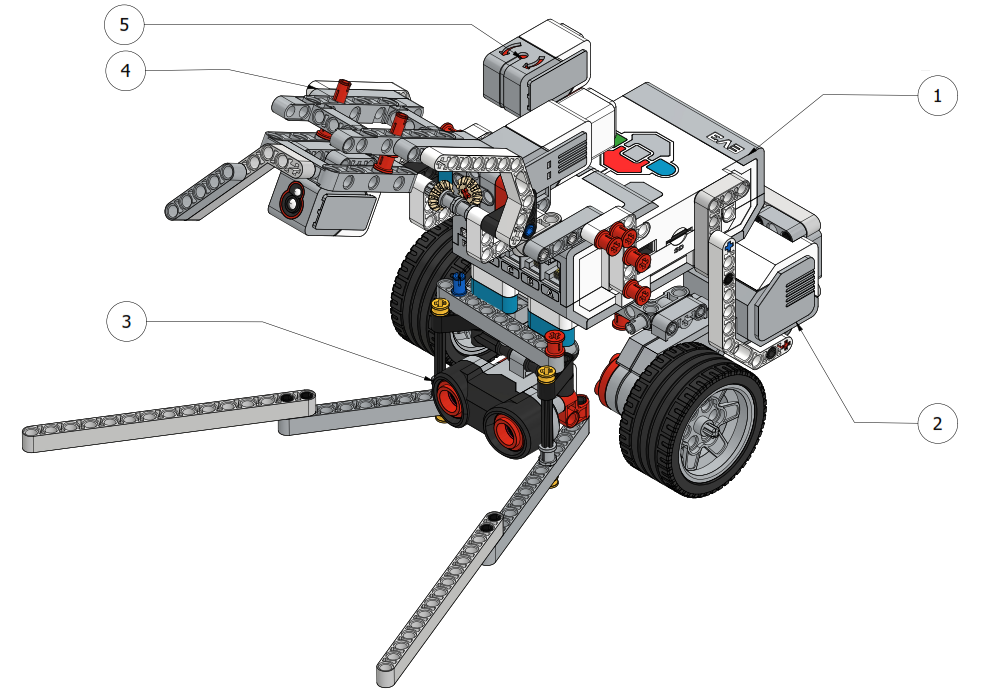
\includegraphics[width=0.8\linewidth]{Graphics/LabelledFruta}
	\caption{Main Components of Fruta Oes}
	\label{fig:labelledfruta}
\end{figure}

\noindent The five main components of this robot are listed in \vref{tab:mechanicalComponents}. \textbf{Item 1-EV3 Brick} is the heart and brain of the robot, the processing of the software takes place in this module. \textbf{Item 2-Drive Base} serves two purposes; providing stability and mobility, the in-depth design of this module will be discussed in \vref{sec:DriveBase}.

	\begin{table}[!ht]
	\centering
	\caption{Main Components}
	\vspace{-2mm}
	\label{tab:mechanicalComponents}
		\begin{tabular}{cl}
			\hline
			\textbf{Item}&\textbf{Component}\\
			\hline
			1&EV3 Brick\\
			2&Drive Base\\
			3&Object Detection and Manipulator Module\\
			4&Gripper and Colour Sensing Module\\
			5&Gyro-Sensor\\
			\hline			
		\end{tabular}
\end{table}

\noindent \textbf{Item 3-Object Detection and Manipulator Module} not only enable object detection capabilities but also makes sure that the object is manipulated to be in a good position for the gripping action. Object Detection and Manipulator Module will be fully discussed in \vref{sec:ObjectDetectionAndHandling}. \textbf{Item 4-Gripper and Colour Sensing Module} grips the object and makes sure it is in a good position for the colour sensor.
\noindent 
\subsection{Object Detection and Manipulator Module}\label{sec:ObjectDetectionAndHandling}

\noindent This section discusses the object detection mechanism. This module not only enable object detection capabilities but also makes sure that the object is manipulated to be in a good position for the gripping action. 
\begin{figure}[!ht]
	\centering
	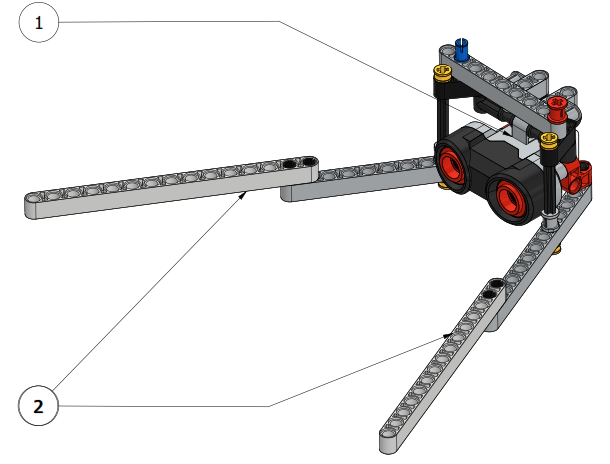
\includegraphics[width=0.8\linewidth]{Graphics/ObjectDetection}
	\caption{Object Detection and Manipulator Module}
	\label{fig:objectDetection}
\end{figure}

\begin{table}[!ht]
	\centering
	\caption{Object Detection and Manipulator Module Components}
	\vspace{-2mm}
	\label{tab:ObjectDetectionComponents}
	\begin{tabular}{cl}
		\hline
		\textbf{Item}&\textbf{Component}\\
		\hline
		1&Ultra Sonic Sensor\\
		2&Manipulator Fangs\\
		\hline			
	\end{tabular}
\end{table}

\noindent \Vref{fig:objectDetection} shows the object detecting manipulator, it is composed of two main parts listed in \vref{tab:ObjectDetectionComponents}: the ultrasonic Sensor which enables the fruit detection capability for the robot and the manipulator fangs. The ultra-sonic sensor is positioned as low as possible, because the objects to be detected are of 2.5cm height. This sensor is also used to provide distances to the robot as it is also capable of computing the distance to the detected object. The EV3 sensor has a measuring range of 250 cm and an accuracy range of $\pm$ 1cm. During the testing phase of the sensors, it was noted that the sensor is sometimes losing the object when the robot is approaching the detected object, this lead to the introduction of the manipulator fangs which are just LEGO beams positioned in such a way that they manipulate the object to slide and ends up in-front of the sensor. This mechanism improved the object detection and made the gripping operation and colour sensing easier. The latter will be discussed later in the document.


\newpage
\subsection{Gripper and Colour Sensing Module}\label{sec:Gripper}

\noindent This section presents the design of the colour sensing and gripping mechanism. This module is also equipped with manipulating fangs. This module is designed to with two states, opened and closed, the module must be fully opened during the searching of fruits in the acre to avoid distracting the signal of the ultrasonic sensor module that was discussed in \vref{sec:ObjectDetectionAndHandling}.
\begin{figure}[!ht]
	\centering
	\begin{subfigure}[b]{0.45\textwidth}
		\centering
		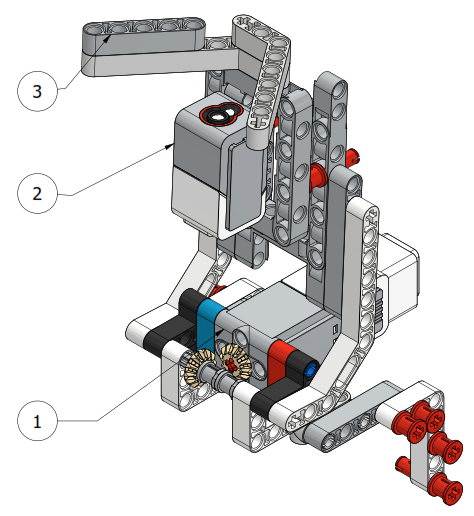
\includegraphics[width=\textwidth]{Graphics/OpenedGripper}
		\caption{Opened Gripper}
		\label{fig:OpenedGripper}
	\end{subfigure}
	~
	\begin{subfigure}[b]{0.45\textwidth}
		\centering
		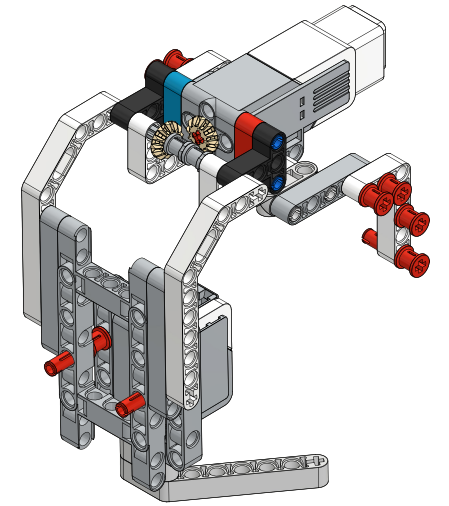
\includegraphics[width=\textwidth]{Graphics/ClosedGripper}
		\caption{Closed Gripper}
		\label{fig:ClosedGripper}
	\end{subfigure}
	\caption{Gripper and Colour Sensing Module}
	\label{fig:gripper}
\end{figure}

\begin{table}[!ht]
	\centering
	\caption{Gripper and Colour Sensing Module Components}
	\vspace{-2mm}
	\label{tab:ColourSensingComponents}
	\begin{tabular}{cl}
		\hline
		\textbf{Item}&\textbf{Component}\\
		\hline
		1&EV3 medium servo motor\\
		2&EV3 Colour Sensor\\
		3&Gripper Manipulator fangs\\
		\hline			
	\end{tabular}
\end{table}


\noindent \Vref{fig:gripper} depicts te gripper and the colour sensing module. \vref{fig:OpenedGripper} shows the gripper in opened mode and \vref{fig:ClosedGripper} shows the gripper in closed mode. This module comprises of three major components: EV3 medium servo motor, this motor is a great solution when the design of the robot requires shorter response times like the harvesting robot designed in this project. The motor is used for opening and closing mechanism of the gripper, it is equipped with 240 to 250 rpm and 0.08 Nm of running torque. The next component is an EV3 Colour sensor, the main function of this component is to enable the robot to distinguish between the required fruits and non-required fruits. The EV3 Colour Sensor is capable of detecting seven colours plus the absence of colour. It can tell the difference between colour or black-and-white or among blue, green, yellow, red, white, and brown. This sensor samples at a rate of 1 kHz, it must be positioned 1cm away from the object for better results.
\newpage
\subsection{Drive Base}\label{sec:DriveBase}

\noindent In this section, the assembling of the drive base for the robot is discussed. it is made up of two parts: EV3 large motors and the wheels, also listed in \vref{tab:DriveBaseComponents}. there is also a balancing wheel positioned underneath the base close to the rear but this wheel is not shown in \vref{fig:DriveBase}.

\begin{figure}[!ht]
	\centering
	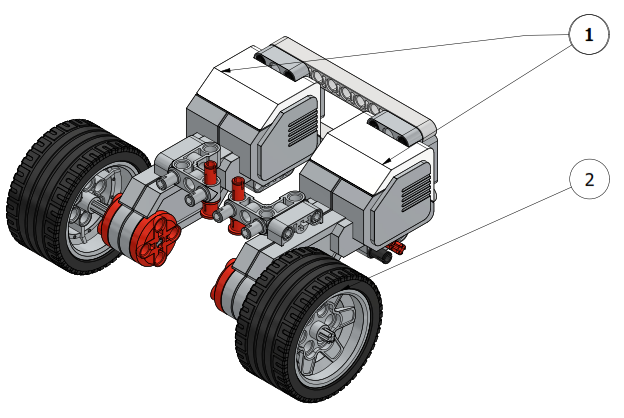
\includegraphics[width=\linewidth]{Graphics/DriveBase}
	\caption{Drive Base}
	\label{fig:DriveBase}
\end{figure}

\begin{table}[!ht]
	\centering
	\caption{Drive Base Components}
	\vspace{-2mm}
	\label{tab:DriveBaseComponents}
	\begin{tabular}{cl}
		\hline
		\textbf{Item}&\textbf{Component}\\
		\hline
		1&EV3 Large Motors\\
		2&Wheels\\
		\hline			
	\end{tabular}
\end{table}

\noindent The EV3 Large Servo Motor uses tacho feedback for accurate control to within one degree \cite{raisingRobots}. 

\newpage
\section{Software Design}\label{sec:softwareDesign}

\subsection{Main Code}\label{sec:mainCode}

\begin{figure}[!ht]
	\centering
	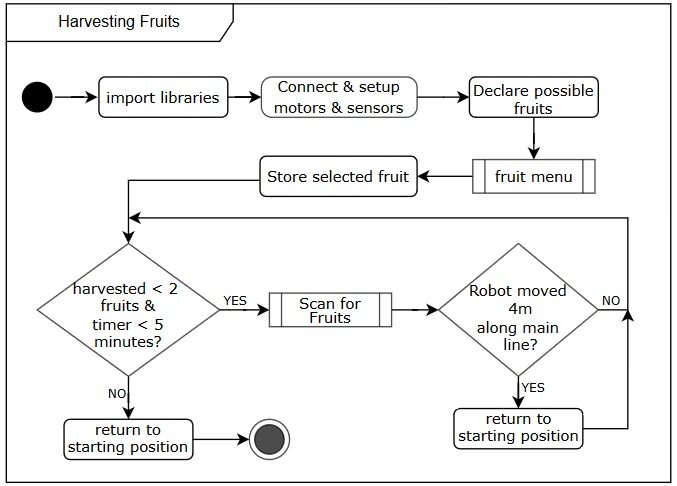
\includegraphics[width=\linewidth]{Graphics/mainCodeActivityDiagram2}
	\caption{Main Code Activity Diagram}
	\label{fig:MainCodeActivityDiagram}
\end{figure}

\newpage
\subsection{User Menu for Selecting the Colour (fruit)}\label{sec:menuCode}

\noindent As it can be seen in \vref{fig:2oppositeviews}, the EV3 brick buttons are coloured with all possible colours of the project: Left button for Blue, Up button for Red and right button for green. The user must wait for the beep after the robot asked them to select the colour from the buttons. Based on the pressed button, the robot will confirm the chosen colour and proceed to search for that specific fruit in the acre. \Vref{fig:menuCodeActivityDiagram} presents the activity diagram for User Menu function, the corresponding source code is attached on appendix B.

\begin{figure}[!ht]
	\centering
	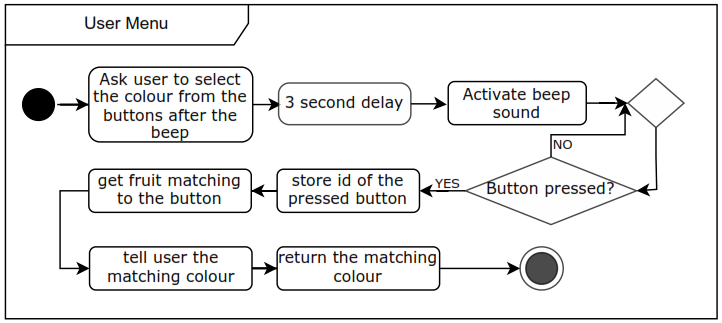
\includegraphics[width=\linewidth]{Graphics/menuCodeActivityDiagram}
	\caption{Menu Code Activity Diagram}
	\label{fig:menuCodeActivityDiagram}
\end{figure}

\noindent \Vref{menuPseudo} presents a pseudo code for this user menu method. A five minute timer is started at the beginning of the function, because one of the requirements is that the robot must return to the starting position after five minutes and this time must be measured as soon as the robot starts interacting with the user. This algorithm is constructed from the activity diagram above.

\begin{algorithm}
	\caption{: User Menu Method Pseudo Code}\label{menuPseudo}
	\begin{algorithmic}[1]
		\State Start the 5 minutes timer;
		\State Use EV3 Speaker function to ask the user to select the colour from the buttons after the beep;
		\State sleep for 3 seconds to allow the sound command to complete;
		\State Activate the EV3 Beep Sound;
		\While{\textit{True}}
		\If{Any button is pressed}
		\State Store the id of the pressed button;
		\State break out of the while loop;
		\EndIf
		\EndWhile
		\State Use the id of the pressed button to get matching fruit from the fruit dictionary;
		\State Use EV3 speaker to tell the user the matching colour;
		\State Return the matching colour to the rest of the code;
	\end{algorithmic}
\end{algorithm}




\newpage
\section{Agile Software Engineering}\label{sec:softwareEngineering}
\subsection{Project Setup} \label{sec:projectSetup}
\noindent LEF BOTS GmbH is a robot specialising company, the name of the firm is created from the initials of the stakeholders: \textbf{L}aura; \textbf{E}ncarnacion; \textbf{F}erlando \textbf{(LEF)}. In this text, the firm presents the development of its major product; the fruit harvesting robot. The robot is given an intuitive name \textbf{Fruta Oes}, which is a combination of two languages Spanish and Afrikaans. Fruta means fruits in Spanish and Oes means to harvest in Afrikaans, thus, the name of the robot \textbf{Fruta Oes} means fruits harvester. One might be asking themselves why Spanish and Afrikaans, well the answer is simple, the stakeholders of the firm are from Spain (Laura and Encarnacion) and South Africa (Ferlando). \Vref{fig:2oppositeviews} Presents \textbf{Fruta Oes}. 

\subsubsection{Project Vision}

"For harvesters who care for the environment. We believe in a world where harvesters can harvest being eco-friendly" 


\subsubsection{SCRUM Team}
\noindent \Vref{fig:scrumTeam} presents the scrum team: Encarnacion Nunez-Ortega is the \textbf{Product Owner} and responsible for determining what needs to be done. Laura Ponce-Orozco is the team's \textbf{Scrum master} and responsible for removing all impediments. The \textbf{development team} consist of Ferlando Mkiva, Encarnacion Nunez-Ortega and Ponce-Orozco together will determine how to deliver chunks of work in frequent increments.
\begin{figure}[!ht]
	\centering
	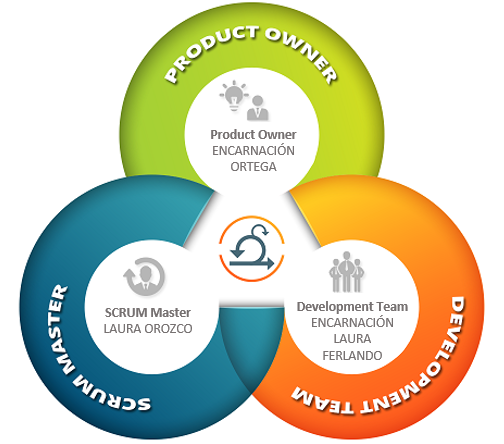
\includegraphics[width=0.6\linewidth]{Graphics/scrumTeam}
	\caption{SCRUM Team}
	\label{fig:scrumTeam}
\end{figure}

\newpage
\subsubsection{Product Backlog}\label{sec:projectBacklog}
\begin{table}[!ht]
	\centering
	\caption{Product Backlog}
	\label{tab:productBacklog}
	\begin{tabular}{c p{30.645em} c}
		\toprule
		\textbf{Priority}&\multicolumn{1}{l}{\textbf{User Story}} & \textbf{Effort} \\
		\midrule
		1&As a user, I want the robot to be completely autonomous. & \adjustimage{height=0.6cm,valign=m}{Graphics/effort1} \\
		\midrule
		2&As a user, I want the robot to ask me for the correct fruit and to confirm that it understood me. & \adjustimage{height=0.6cm,valign=m}{Graphics/effort2} \\
		\midrule
		3&As a developer, I want the robot to be able to detect a 2.5cm cube. & \adjustimage{height=0.6cm,valign=m}{Graphics/effort1} \\
		\midrule
		4&As a user, I want the robot to look for the specified fruit and check if the fruit is correctly grabbed. & \adjustimage{height=0.6cm,valign=m}{Graphics/effort5}\\
		\midrule
		5&As a user, I don’t want the robot to return to the home zone without the fruit grabbed. & \adjustimage{height=0.6cm,valign=m}{Graphics/effort4} \\
		\midrule
		6&As a user, I want the robot to place the right fruit in the home zone. & \adjustimage{height=0.6cm,valign=m}{Graphics/effort3} \\
		\midrule
		7&As a developer, I want the robot to keep count of the harvested fruits & \adjustimage{height=0.6cm,valign=m}{Graphics/effort1} \\
		\midrule
		8&As a user, I want the robot to immediately return to the starting point after collecting two fruits within 5 minutes. & \adjustimage{height=0.6cm,valign=m}{Graphics/effort4} \\
		\midrule
		9&As a user, I don’t want the robot to search for fruits outside the acre. & \adjustimage{height=0.6cm,valign=m}{Graphics/effort3} \\
		\midrule
		10&As a developer, I want the code to be efficient.  & \adjustimage{height=0.6cm,valign=m}{Graphics/effort4} \\
		\bottomrule
	\end{tabular}%
\end{table}%

\newpage
\subsection{Sprint 1} \label{sec:sprint1}
\subsubsection{Goals of the sprint}\label{sec:sprint1goals}
\noindent The goal of this sprint was to tackle the following user stories. In total five cups of coffees must be consumed as the effort of this sprint.\\
~\\
\begin{minipage}[t]{0.35\textwidth}
	\begin{StickyNote}[Priority 2]
		As a \textbf{user}, I want the robot to ask me for the \textbf{correct fruit} and to confirm that it understood me.
		\adjustimage{height=0.6cm,valign=m}{Graphics/effort22}
	\end{StickyNote}
\end{minipage}
\begin{minipage}[t]{0.3\textwidth}
		\begin{StickyNote}[Priority 3]
		As a \textbf{developer}, I want the robot to be able to \textbf{detect} a 2.5cm cube.
		\adjustimage{height=0.6cm,valign=m}{Graphics/effort12}
	\end{StickyNote}
\end{minipage}
\begin{minipage}[t]{0.35\textwidth}
	\begin{StickyNote}[Priority 4]
	As a \textbf{user}, I want the robot to look for the \textbf{specified fruit} and check if the fruit is correctly grabbed.
	\adjustimage{height=0.6cm,valign=m}{Graphics/effort22}
\end{StickyNote}
\end{minipage}

\subsubsection{Burn-down Chart}\label{sec:sprint1bdc}
\begin{figure}[H]
	\centering
	\begin{tikzpicture}
		\begin{axis}
			[
			legend pos=north east,
			every axis plot/.append style={ultra thick},
			xmin = 0,
			ymin = 0,
			xmajorgrids=true,
			grid style=dashed,
			width=0.8\textwidth,
			height=0.5\textwidth,
			xlabel=\textbf{Days},
			ylabel=\textbf{Coffees \adjustimage{height=0.6cm,valign=m}{Graphics/effortN}},
			y tick label style={
				/pgf/number format/.cd,
				fixed,
				fixed zerofill,
				precision=0,
				/tikz/.cd
			},
			x tick label style={
				/pgf/number format/.cd,
				fixed,
				fixed zerofill,
				precision=0,
				/tikz/.cd
			},
			scaled ticks=false,
			yticklabel={${\pgfmathprintnumber{\tick}}$},
			]
			\addlegendimage{empty legend}
			\addplot[orange, mark=none] table[x index=0, y index=1, col sep=comma] {Sprint1.csv};
			\addplot[green, mark=none] table[x index=2, y index=3, col sep=comma] {Sprint1.csv};
			\addlegendentry{\hspace{-.6cm}\textbf{Burn-down Charts}}
			\addlegendentry{Actual}
			\addlegendentry{Ideal}
		\end{axis}
	\end{tikzpicture}
	\vspace{-1mm}
	\caption{Sprint 1 Burnd-own Chart}
	\label{fig:sprint1BurndownChart}
\end{figure}

\newpage
\subsection{Sprint 2}	\label{sec:sprint2}

\subsubsection{Goals of the sprint}\label{sec:sprint2goals}
\noindent The goal of this sprint was to tackle the following user stories. In total five cups of coffees must be consumed as the effort of this sprint.\\
~\\
\begin{minipage}[t]{0.21\textwidth}
	\begin{StickyNote}[Priority 2]
		As a \textbf{user}, I want the robot to place the right fruit in the home zone.
		\adjustimage{height=0.6cm,valign=m}{Graphics/effort32}
	\end{StickyNote}
\end{minipage}
\begin{minipage}[t]{0.24\textwidth}
	\begin{StickyNote}[Priority 3]
		As a user, I don’t want the robot to return to the home zone without the fruit grabbed.
		\adjustimage{height=0.6cm,valign=m}{Graphics/effort12}
	\end{StickyNote}
\end{minipage}
\begin{minipage}[t]{0.26\textwidth}
	\begin{StickyNote}[Priority 4]
		As a user, I want the robot to look for the specified fruit and check if the fruit is correctly grabbed.
		\adjustimage{height=0.6cm,valign=m}{Graphics/effort22}
	\end{StickyNote}
\end{minipage}
\begin{minipage}[t]{0.26\textwidth}
	\begin{StickyNote}[Priority 4]
		As a user, I want the robot to look for the specified fruit and check if the fruit is correctly grabbed.
		\adjustimage{height=0.6cm,valign=m}{Graphics/effort22}
	\end{StickyNote}
\end{minipage}

\subsection{Sprint 3} \label{sec:sprint3}

\section{Recommendations and Conclusion} \label{sec:RecommendationsAndConclusion}


